\section{Benchmark Ablation and Cross-Domain Stability Analysis}
\label{sec:phase2}

Before extending KAN-ODE to new systems, two questions needed settling: which
solver and basis choices this architecture actually prefers, and whether the
baseline recipe (Section~\ref{sec:phase1}) transfers unchanged to systems
beyond Lotka-Volterra. Both were answered empirically, and the second
uncovered two genuine training failures that required a mechanistic diagnosis
before they could be fixed.

\subsection{Solver, basis and architecture ablation}

Table~\ref{tab:solver-ablation} sweeps six explicit Runge-Kutta integrators at
fixed radial-basis-function (RBF) basis; Table~\ref{tab:basis-ablation}
sweeps seven basis representations at fixed Tsit5 solver. Both use the
protocol of Section~\ref{sec:phase1}. The number of function evaluations per
training epoch (how many times the integrator must call the network per
step) is reported because it is the dominant cost driver for training time.
The Lipschitz constant $L$ of the trained field -- an upper bound on how much
the output of $\mathbf{f}_\theta$ can change per unit change of its input,
estimated numerically from the trained weights -- is reported alongside
accuracy because it is a direct measure of how smooth or jagged the basis
expansion in Equation~\ref{eq:kan-edge} ended up, independent of the
trajectory error.

\begin{table}[!ht]
\centering
\footnotesize
\renewcommand{\arraystretch}{1.1}
\caption{Solver ablation (fixed RBF basis, $\Delta t=0.1$, 240 parameters).}
\label{tab:solver-ablation}
\begin{tabularx}{\textwidth}{@{}L{2.3cm} C{1.0cm} C{1.6cm} C{1.7cm} C{1.9cm} C{1.9cm} X@{}}
\toprule
\hdrrow \thh{Solver} & \thh{Order} & \thh{Function evaluations / epoch} & \thh{Training MSE} & \thh{Extrapolation MSE} & \thh{Extrapolation $R^2$} & \thh{Lipschitz $L$}\\
\midrule
Forward Euler & 1 & 70 & $1.38\times10^{-4}$ & $2.51\times10^{-3}$ & $0.99914$ & $8.55$\\
Heun RK2 & 2 & 140 & $8.32\times10^{-5}$ & $3.10\times10^{-4}$ & $0.99989$ & $7.07$\\
Midpoint & 2 & 140 & $8.86\times10^{-5}$ & $8.95\times10^{-5}$ & $0.99997$ & $6.96$\\
Classical RK4 & 4 & 280 & $9.41\times10^{-5}$ & $9.29\times10^{-5}$ & $0.99997$ & $6.88$\\
DOPRI5 & 5 & 420 & $9.28\times10^{-5}$ & $9.21\times10^{-5}$ & $0.99997$ & $6.89$\\
\textbf{Tsit5} & 5 & 420 & $\mathbf{8.83\times10^{-5}}$ & $\mathbf{8.92\times10^{-5}}$ & $\mathbf{0.99997}$ & $6.91$\\
\bottomrule
\end{tabularx}
\end{table}

Truncation error dominates only at order $p=1$: Euler's extrapolation MSE is
$28\times$ Tsit5's, and it is the only solver that fails to reach $10^{-4}$
training loss within budget. Its trained field is also the least smooth of
the six ($L=8.55$, the highest in the table), consistent with a systematic
bias forcing the network to fit a sharper correction than the smoother
integrators require. Above order 2 the ranking collapses into a $3.8\%$
spread with no monotonic order dependence -- at $\Delta t=0.1$, integrator
truncation error has fallen below the optimization noise floor. Midpoint
matches Tsit5's accuracy within $0.3\%$ at one third of the function
evaluations, making it the cost-normalized optimum on this problem.

\begin{table}[!ht]
\centering
\footnotesize
\renewcommand{\arraystretch}{1.1}
\caption{Basis ablation (fixed Tsit5 solver, $G=5$ grid points, 240 parameters).}
\label{tab:basis-ablation}
\begin{tabularx}{\textwidth}{@{}L{2.1cm} C{1.9cm} C{2.0cm} C{1.1cm} C{1.6cm} X@{}}
\toprule
\hdrrow \thh{Basis function} & \thh{Training MSE} & \thh{Extrapolation MSE} & \thh{$R^2$} & \thh{Lipschitz $L$} & \thh{Wall-clock time}\\
\midrule
Cubic B-spline & $\mathbf{7.20\times10^{-5}}$ & $\mathbf{8.38\times10^{-5}}$ & $\mathbf{0.99997}$ & $8.44$ & 6680 seconds\\
Gaussian RBF & $8.83\times10^{-5}$ & $8.92\times10^{-5}$ & $0.99997$ & $6.91$ & \textbf{1712 seconds}\\
Chebyshev & $9.80\times10^{-5}$ & $4.37\times10^{-4}$ & $0.99985$ & $6.48$ & 2317 seconds\\
Lagrange & $1.07\times10^{-4}$ & $3.93\times10^{-4}$ & $0.99987$ & $6.70$ & 6829 seconds\\
Newton & $1.47\times10^{-3}$ & $3.65\times10^{-2}$ & $0.98746$ & $5.65$ & 2187 seconds\\
\bottomrule
\end{tabularx}
\end{table}

B-spline edges out RBF on accuracy after a boundary-knot fix, at $3.9\times$
RBF's wall-clock time and a visibly higher Lipschitz constant ($8.44$ vs.\
$6.91$) -- its compact local support (Equation~\ref{eq:kan-edge}'s $B_i(x)$
vanishing outside each knot span) lets it fit sharper local features than
RBF's smooth global support without being penalized elsewhere in the domain.
The two bases are statistically tied on error (6\% apart, inside
single-seed noise), which makes RBF the better accuracy-per-second choice.
Polynomial global-support bases (Chebyshev, Lagrange) fit the training
window well and extrapolate $4$--$5\times$ worse -- the expected signature
of a basis whose every coefficient influences the whole domain rather than a
local region of it. Newton's basis is the outlier on smoothness in the
opposite direction: its lowest Lipschitz constant in the table ($5.65$)
reflects underfitting, not desirable flatness, since it is also the only
basis that never reaches $10^{-3}$ training loss.

A parameter-matched comparison against a standard multilayer perceptron
(MLP) trained as a Neural ODE found KAN-ODE extrapolates $5.4\times$ better
than the MLP from statistically identical training loss, while the MLP
converges $4.1\times$ \emph{faster} to $10^{-3}$ loss. This directly
contradicts the base paper's own headline efficiency claim on this same
system -- a $10^4$-epoch KAN-ODE against a $10^5$-epoch, parameter-matched
MLP-ODE, a tenfold speed advantage the paper attributes to the network
(Section~\ref{sec:introduction}). Under this project's protocol, at matched parameter count (240 vs.\ 252) and
matched optimizer settings, the MLP was faster to converge on Lotka-Volterra
rather than slower, though KAN-ODE still won decisively on the extrapolation
accuracy the paper's other headline claim concerns.

\begin{table}[!ht]
\centering
\footnotesize
\renewcommand{\arraystretch}{1.15}
\caption{Controlled breakdown of why the paper's literal MLP baseline
architecture, $[2,50,2]$ with hyperbolic tangent (tanh) activation, fails to
train under this project's protocol. All four runs use 2000 epochs.}
\label{tab:mlp-breakdown}
\begin{tabularx}{\textwidth}{@{}C{0.7cm} L{2.8cm} C{1.4cm} C{1.5cm} C{2.1cm} C{2.1cm} C{1.6cm}@{}}
\toprule
\hdrrow \thh{Run} & \thh{Architecture} & \thh{Activation} & \thh{Learning rate} & \thh{Training MSE} & \thh{Extrapolation MSE} & \thh{$R^2$}\\
\midrule
A & $[2,50,2]$ & tanh & $2\times10^{-3}$ & $1.21\times10^{0}$ & $1.98\times10^{0}$ & $0.319$\\
B & $[2,50,2]$ & tanh & $5\times10^{-4}$ & $1.85\times10^{0}$ & $9.23\times10^{0}$ & $-2.169$\\
C & $[2,14,8,8,2]$ & SiLU & $2\times10^{-3}$ & $\mathbf{4.28\times10^{-4}}$ & $\mathbf{6.97\times10^{-4}}$ & $\mathbf{0.99976}$\\
D & $[2,50,2]$ & SiLU & $2\times10^{-3}$ & $3.62\times10^{-3}$ & $2.68\times10^{2}$ & $-91.06$\\
\bottomrule
\end{tabularx}
\end{table}

Comparing run A against run D, which share the same architecture and differ
only in activation, shows a $335\times$ gap in extrapolation error -- the
activation function determines whether this architecture fits the data at
all. Comparing run C against run D, which share the SiLU activation and
differ only in architecture depth, shows extrapolation error of
$6.97\times10^{-4}$ against $2.68\times10^{2}$ -- network depth determines
extrapolation quality once the activation is fixed to one that trains. This
isolates the activation choice as the specific cause of the paper's literal
architecture failing to train under this project's protocol, independent of
the epoch budget question addressed in Section~\ref{sec:phase4}.

\subsection{Diagnosing and fixing two cross-domain failures}

Applying the Lotka-Volterra recipe unchanged to the damped pendulum and to
SIR failed on both systems, each for its own reason. Both diagnoses follow
the same discipline: measure a quantity about the model's behavior
\emph{before} training rather than search the hyperparameter space after a
failed run.

\paragraph{Pendulum: extending the training window.} The pendulum recipe
originally trained on $t\in[0,3.5]$ and diverged in extrapolation
($R^2=-1.318$). Extending the training window to $t_{\text{train}}=5.0$ --
a single flag -- resolves it:

\begin{expectbox}
\expectrow{Question}{Why does the Lotka-Volterra recipe, applied unchanged, diverge on the pendulum?}
\expectrow{Expected (hypothesis)}{SiLU's residual branch cannot represent the sign-changing derivative $\dot\theta=\omega$ -- an architectural limit.}
\expectrow{Observed}{Refuted. A longer training window fixes it under either activation; SiLU fits the sign change fine once the window is long enough.}
\end{expectbox}

\begin{table}[!ht]
\centering
\footnotesize
\renewcommand{\arraystretch}{1.2}
\caption{Pendulum fix: best configuration versus the original failure.}
\label{tab:pendulum-fix}
\begin{tabularx}{\textwidth}{@{}X C{2.6cm} C{2.2cm} C{1.8cm}@{}}
\toprule
\hdrrow \thh{Configuration} & \thh{Full-horizon MSE} & \thh{Extrapolation $R^2$} & \thh{Verdict}\\
\midrule
Original ($t_{\text{train}}=3.0$) & $8.99\times10^{-1}$ & $-1.318$ & diverges\\
Extended window ($t_{\text{train}}=5.0$, SiLU) & $\mathbf{4.48\times10^{-2}}$ & $\mathbf{+0.647}$ & \textbf{adopted}\\
\bottomrule
\end{tabularx}
\end{table}

An earlier hypothesis held that SiLU's residual branch $W\cdot\mathrm{silu}(x)$
cannot represent a sign-changing derivative such as $\dot\theta=\omega$. A
factorial control comparing activation against training-window length
refutes it directly: with the longer window, SiLU reaches an angular-velocity
root-mean-square error of $0.0114$ radians and reproduces the true turning
point ($\theta_{\min}=-1.380$ against a true value of $-1.385$). The training
window is what fixes the pendulum; the activation choice affects only how
quickly the fit is reached, with the identity activation converging
$\sim\!1000\times$ faster at the short window without matching the longer
window's accuracy.

\begin{figure}[htbp]
\centering
\begin{minipage}[t]{0.48\textwidth}
\centering
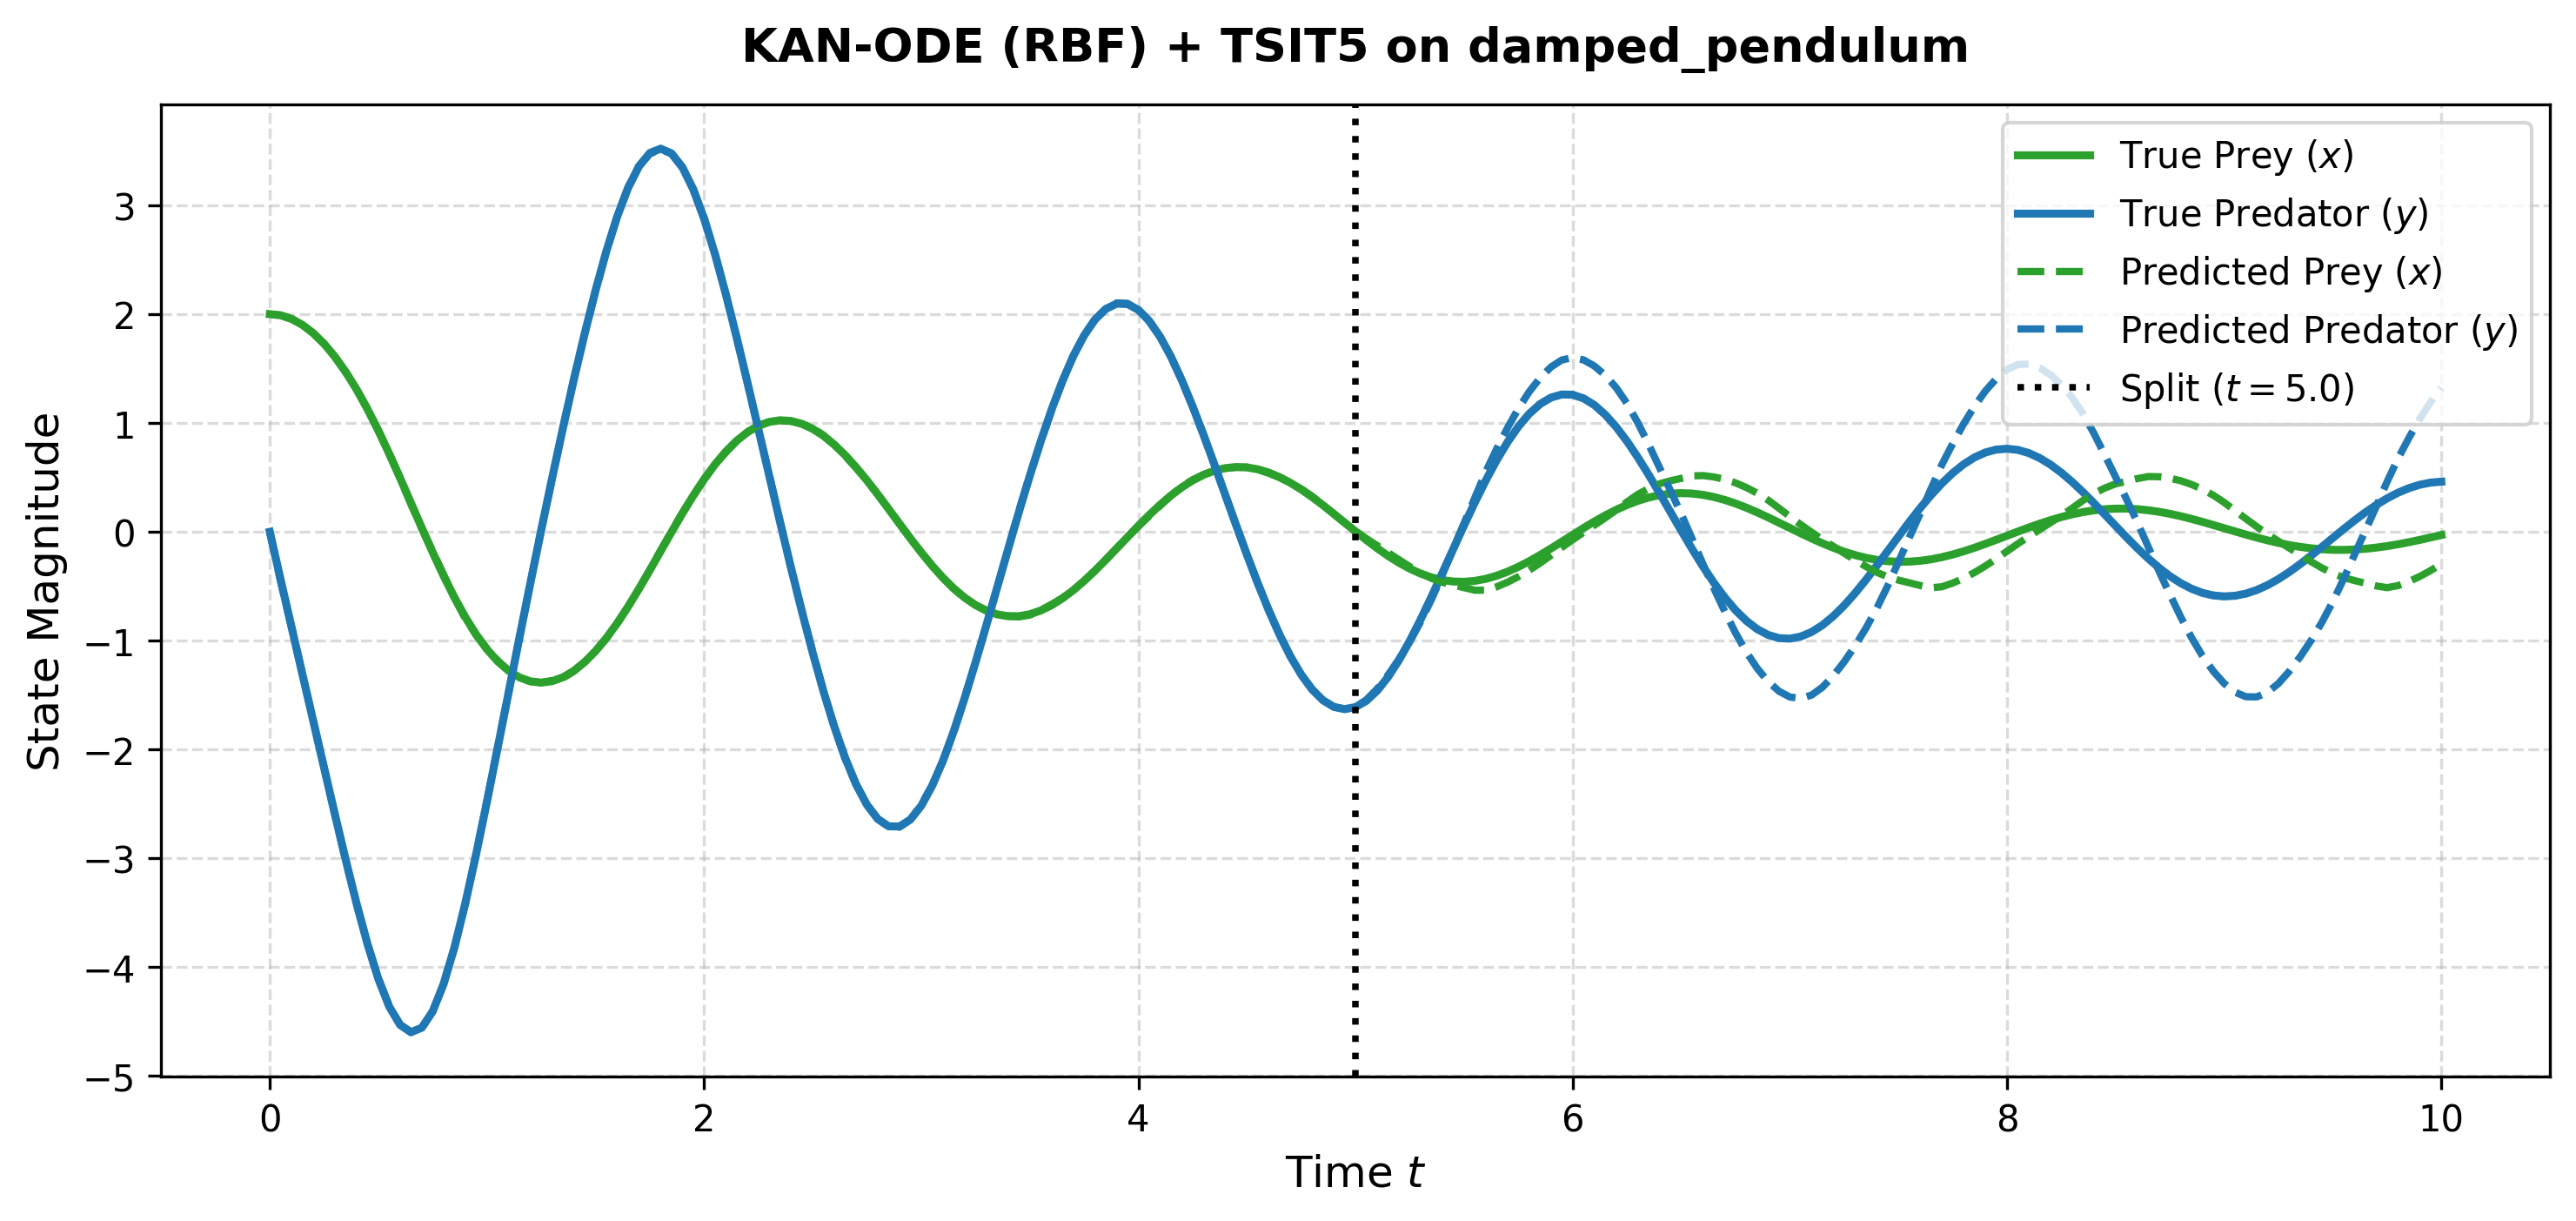
\includegraphics[width=\linewidth]{figures/phase2/pendulum_fixed_trajectory.png}
\end{minipage}\hfill
\begin{minipage}[t]{0.48\textwidth}
\centering
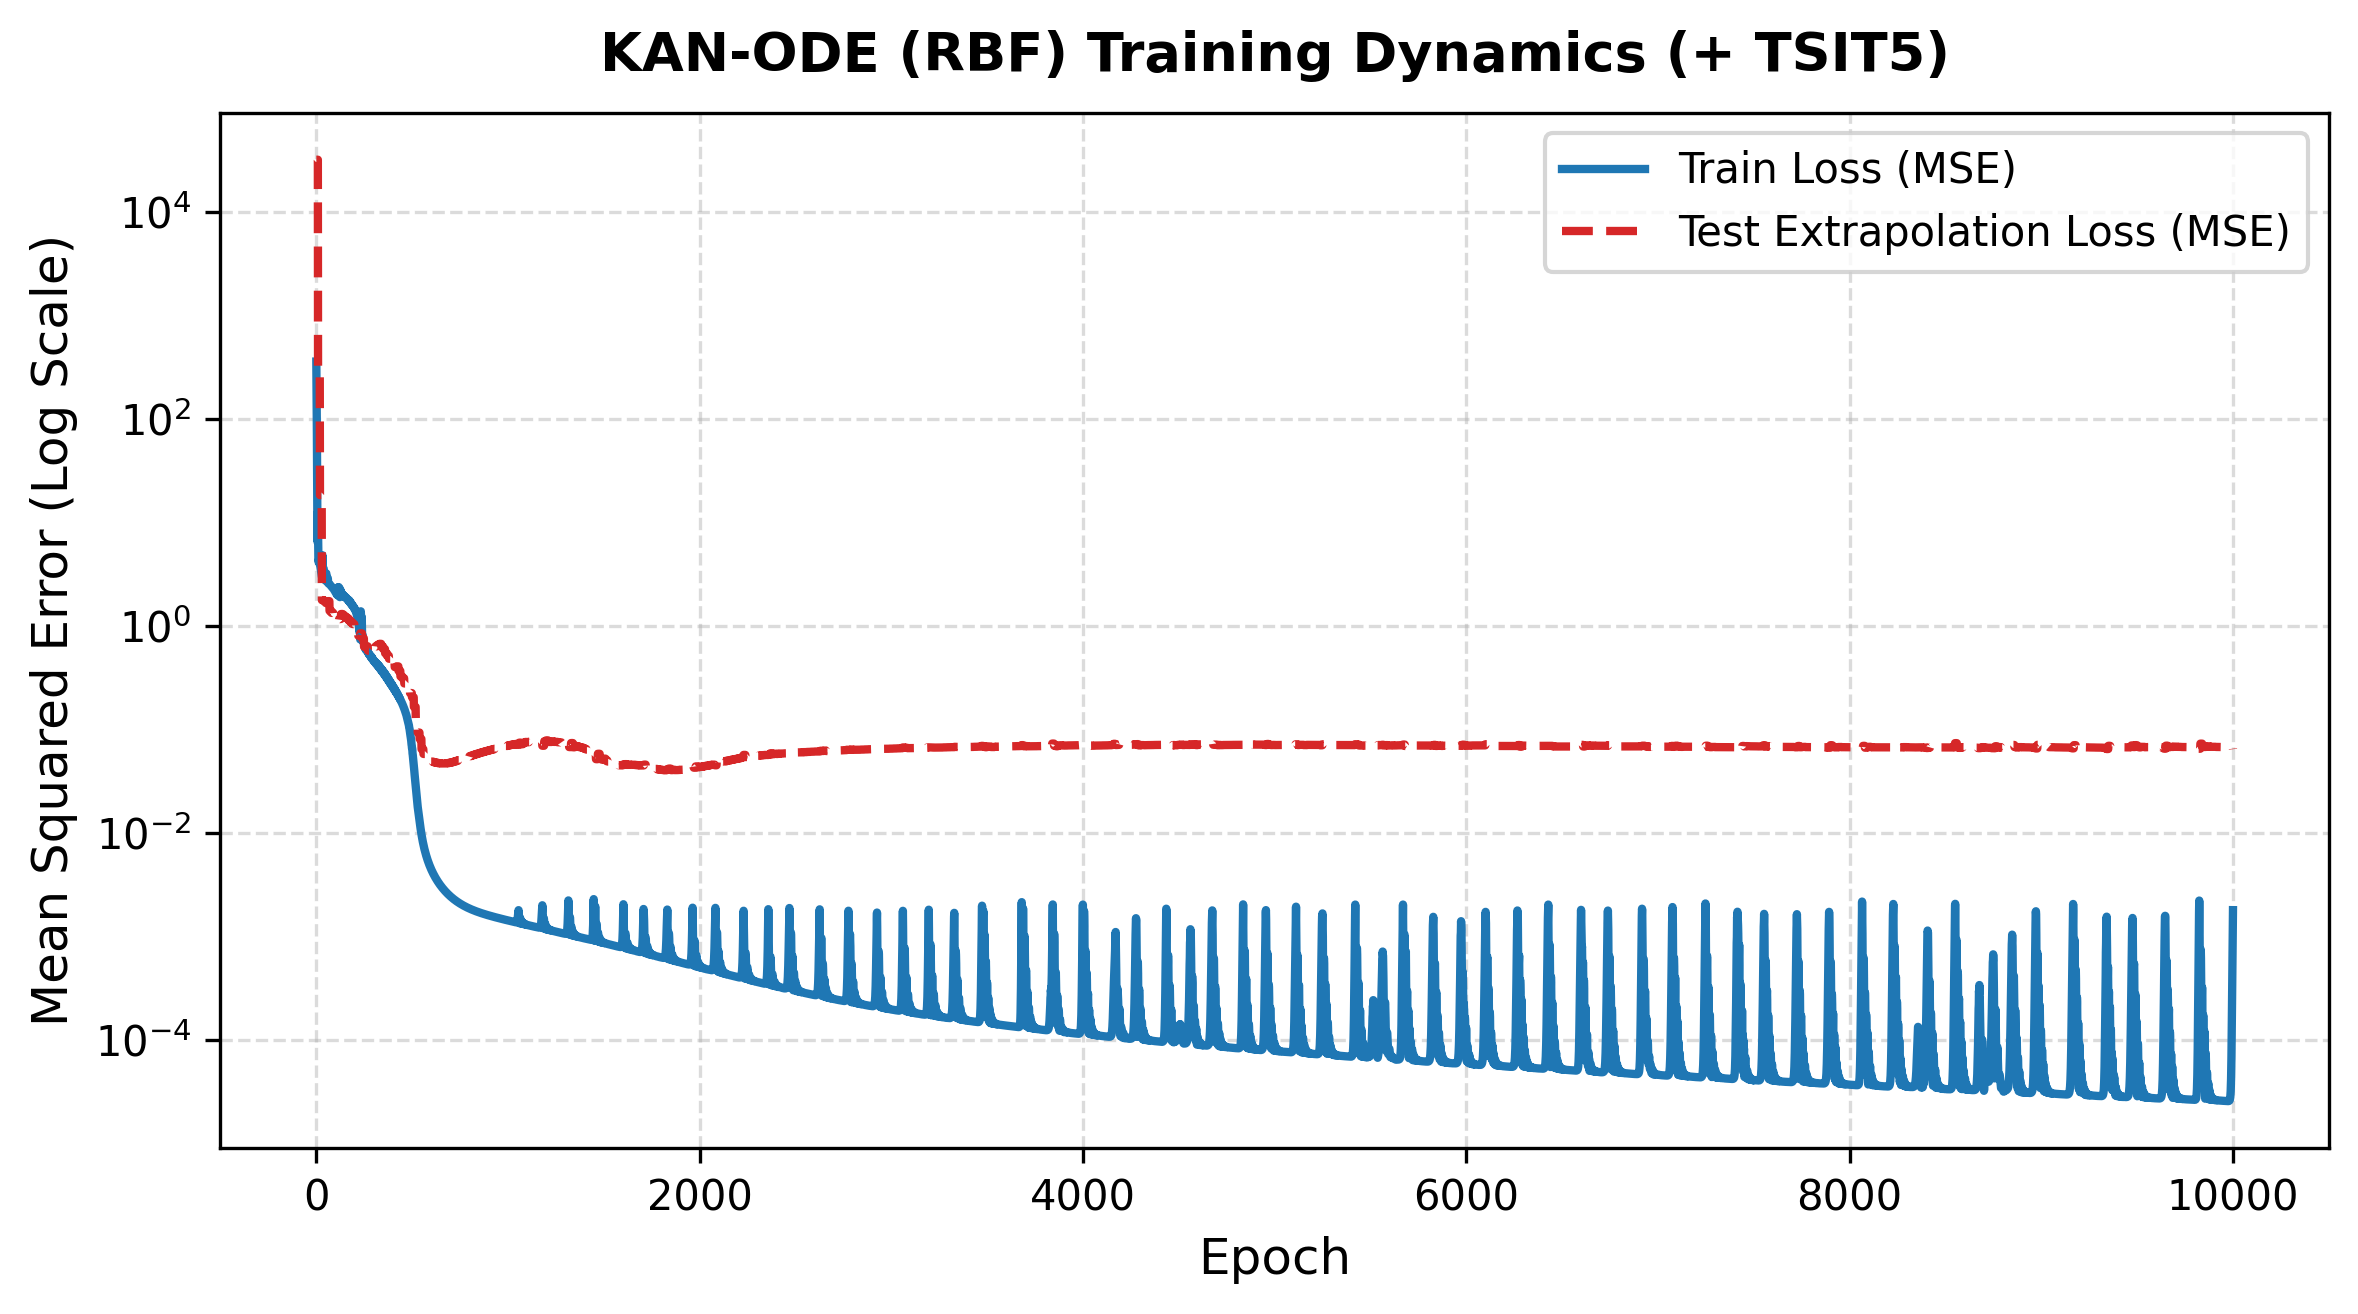
\includegraphics[width=\linewidth]{figures/phase2/pendulum_fixed_loss_curves.png}
\end{minipage}
\caption{Fixed-pendulum trajectory reconstruction (left) and training/extrapolation
loss curves (right), using the extended-window recipe.}
\label{fig:pendulum-fixed}
\end{figure}

\paragraph{SIR: a unit-scale mismatch.} SIR diverged to an invalid
(not-a-number) value at epoch 8686.

\begin{expectbox}
\expectrow{Question}{What causes SIR's divergence, and is it a scale problem, an optimizer defect, or a modeling gap?}
\expectrow{Expected}{Measuring the untrained network's own field magnitude against the true dynamics, before any training, should reveal whether the two are mismatched in scale.}
\expectrow{Observed}{A $19\times$ speed mismatch at initialization. Rescaling time removes the divergence entirely; no optimizer or architecture change was needed.}
\end{expectbox}

Measuring the learned field magnitude
\emph{before any training step} explained it directly: a Glorot-initialised
KAN starts with $|f_\theta|\approx0.203$ against SIR's true field magnitude
of $0.011$ over a training horizon $T=50$ -- a $19\times$ speed mismatch that
makes $f_\theta\to\mathbf{0}$ the steepest local descent direction available.
The optimizer was behaving rationally: collapsing the field to zero genuinely
reduces the loss fastest when the target dynamics evolve this much slower
than the model's initial guess. Rescaling time by a factor of 10 removes the
mismatch; projecting the learned field onto the subspace where the
compartments sum to a constant fixes a separate mass-drift symptom.
Final SIR result: mass error reduced from $5.9\times10^{-2}$ to
$7\times10^{-7}$, extrapolation $R^2=+0.9981$.

\begin{figure}[htbp]
\centering
\begin{minipage}[t]{0.48\textwidth}
\centering
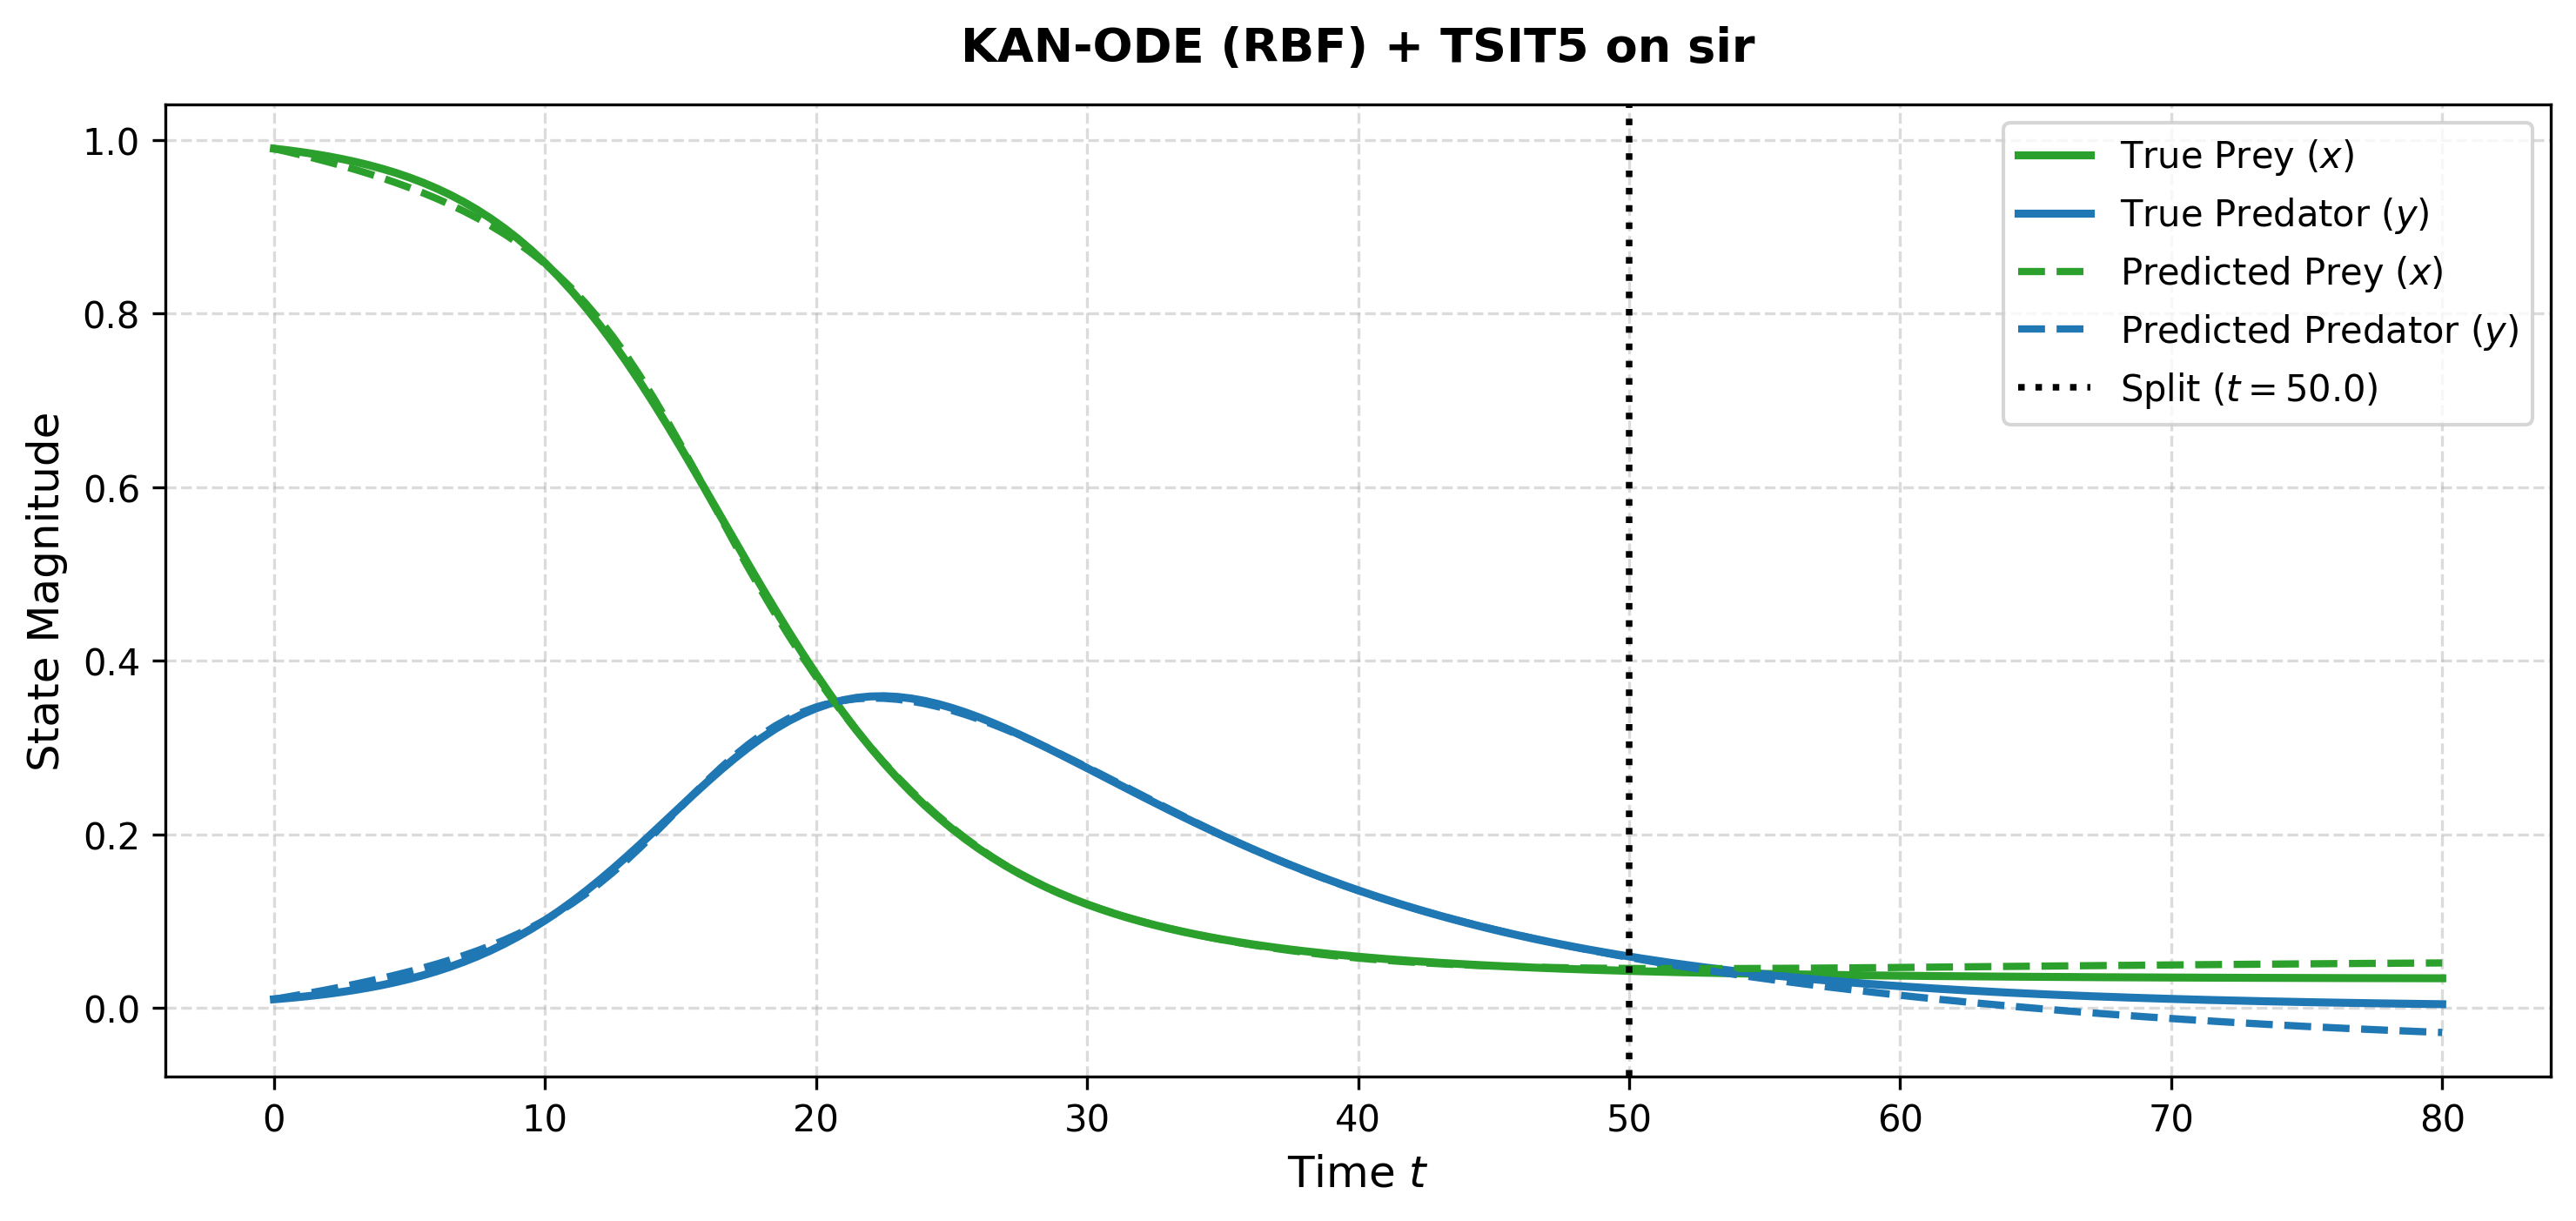
\includegraphics[width=\linewidth]{figures/phase2/sir_fixed_trajectory.png}
\end{minipage}\hfill
\begin{minipage}[t]{0.48\textwidth}
\centering
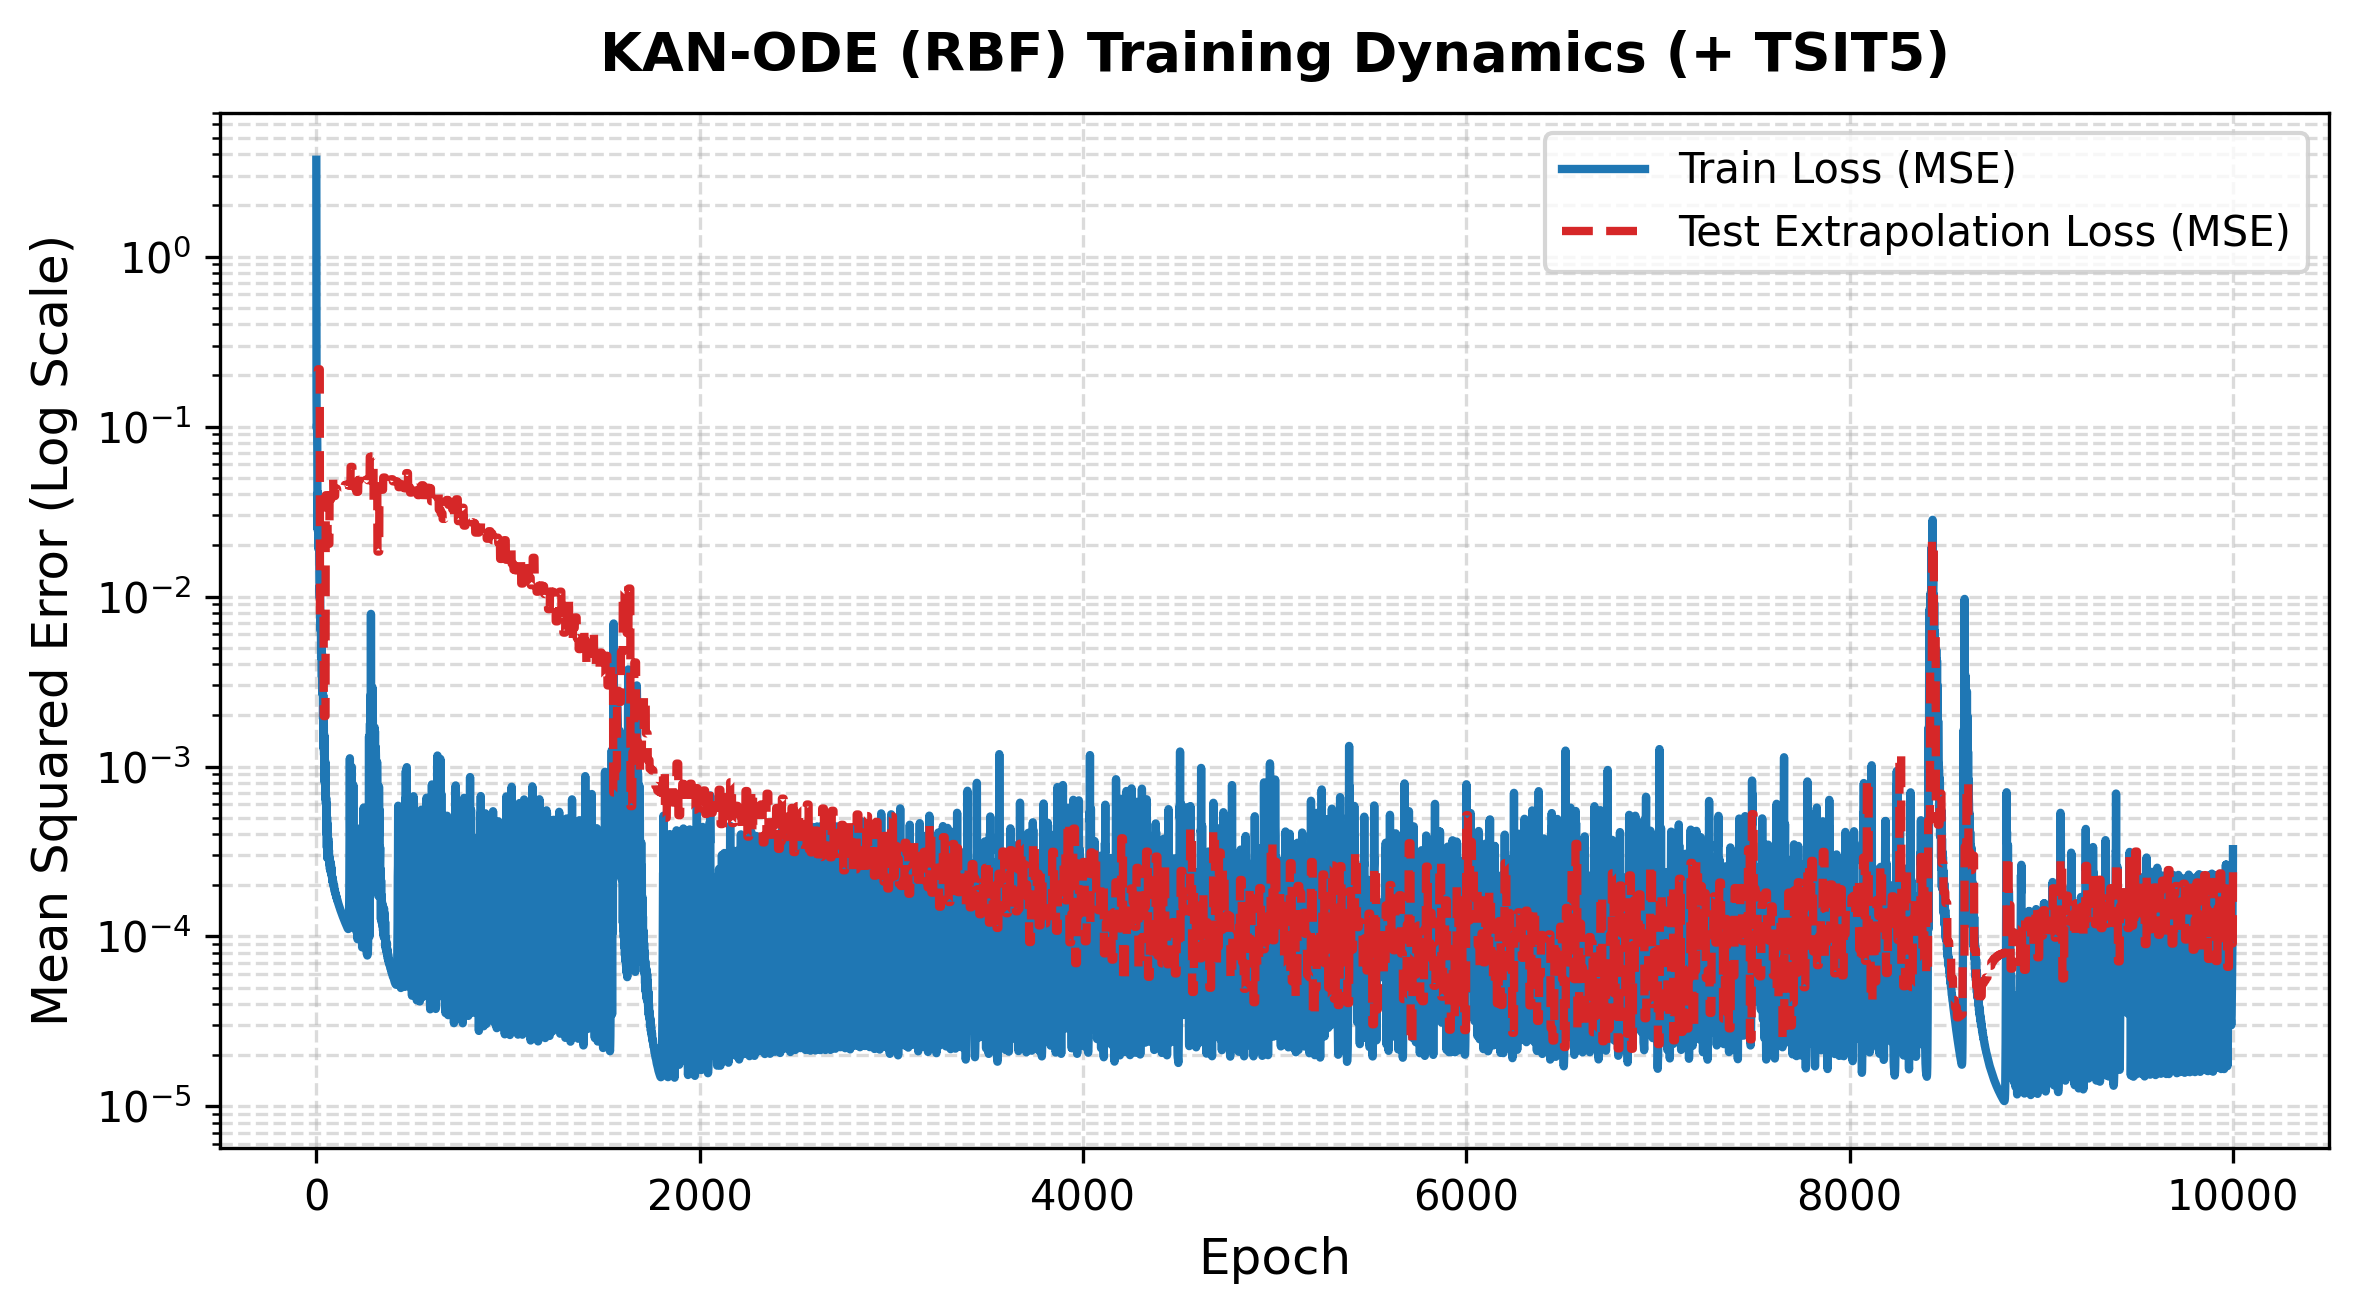
\includegraphics[width=\linewidth]{figures/phase2/sir_fixed_loss_curves.png}
\end{minipage}
\caption{Fixed-SIR trajectory reconstruction (left) and loss curves (right).}
\label{fig:sir-fixed}
\end{figure}

\paragraph{Other fixes considered.} Several additional interventions were
tested and are recorded for completeness rather than adopted:

\begin{table}[!ht]
\centering
\footnotesize
\renewcommand{\arraystretch}{1.15}
\caption{Every stability intervention tested, including the rejected ones.}
\label{tab:fix-scorecard}
\begin{tabularx}{\textwidth}{@{}L{4.4cm} C{2.0cm} X@{}}
\toprule
\hdrrow \thh{Intervention} & \thh{Verdict} & \thh{Evidence}\\
\midrule
Longer training window (pendulum) & Adopted & $R^2$ improves from $-1.318$ to $+0.647$; works for both activations tested\\
Non-finite gradient guard with automatic abort & Adopted & Caught SIR's divergence at epoch 3055, preserved a valid checkpoint instead of overwriting it with an invalid one\\
Time rescaling (SIR) & Adopted & Removes both the divergence and the frozen-field behavior\\
Conservation via subspace projection (SIR) & Adopted & Mass error reduced from $5.9\times10^{-2}$ to $7\times10^{-7}$\\
Identity activation (pendulum) & Speed only & Roughly $1000\times$ faster to fit at the short window, but worse extrapolation and stability at the long window\\
Standard-deviation loss weighting & System-dependent & Worst-performing pendulum option; superseded for SIR by time rescaling\\
Conservation via penalty term & Rejected & Wrong mechanism -- the training window's mass was already close to conserved, so the penalty had nothing to correct\\
Widened basis-function grid limits & Rejected & Performed worse than the untouched baseline configuration\\
\bottomrule
\end{tabularx}
\end{table}

\begin{keypoint}[Methodological lesson carried into every later study]
Both diagnoses came from measuring the learned field's own magnitude at
initialization, before training ever ran. This init-time-measurement
discipline reappears verbatim in the real-epidemic-data test of
Section~\ref{sec:track-e}.
\end{keypoint}

\FloatBarrier
